\documentclass[addpoints,spanish, 12pt,a4paper]{exam}
%\documentclass[answers, spanish, 12pt,a4paper]{exam}
\printanswers
\pointpoints{punto}{puntos}
\hpword{Puntos:}
\vpword{Puntos:}
\htword{Total}
\vtword{Total}
\hsword{Resultado:}
\hqword{Ejercicio:}
\vqword{Ejercicio:}

\usepackage[utf8]{inputenc}
\usepackage[spanish]{babel}
\usepackage{eurosym}
%\usepackage[spanish,es-lcroman, es-tabla, es-noshorthands]{babel}


\usepackage[margin=1in]{geometry}
\usepackage{amsmath,amssymb}
\usepackage{multicol}
\usepackage{yhmath}

\pointsinrightmargin % Para poner las puntuaciones a la derecha. Se puede cambiar. Si se comenta, sale a la izquierda.
\extrawidth{-2.4cm} %Un poquito más de margen por si ponemos textos largos.
\marginpointname{ \emph{\points}}

\usepackage{graphicx}

\graphicspath{{../../img/}} 

\newcommand{\class}{1º Bachillerato CCSS}
\newcommand{\examdate}{\today}
\newcommand{\examnum}{Convocatoria Ordinaria}
\newcommand{\tipo}{A}


\newcommand{\timelimit}{105 minutos}

\renewcommand{\solutiontitle}{\noindent\textbf{Solución:}\enspace}


\pagestyle{head}
\firstpageheader{
\includegraphics[width=0.2\columnwidth]{header_left}}{\textbf{Departamento de Matemáticas\linebreak \class}\linebreak \examnum}{
\includegraphics[width=0.1\columnwidth]{header_right}}
\runningheader{\class}{\examnum}{Página \thepage\ of \numpages}
\runningheadrule


\usepackage{pgf,tikz,pgfplots}
\pgfplotsset{compat=1.15}
\usepackage{mathrsfs}
\usetikzlibrary{arrows}


\begin{document}

\noindent
\begin{tabular*}{\textwidth}{l @{\extracolsep{\fill}} r @{\extracolsep{6pt}} }
\textbf{Nombre:} \makebox[3.5in]{\hrulefill} & \textbf{Fecha:}\makebox[1in]{\hrulefill} \\
 & \\
\textbf{Tiempo: \timelimit} & Tipo: \tipo 
\end{tabular*}
\rule[2ex]{\textwidth}{2pt}
Esta prueba tiene \numquestions\ ejercicios. La puntuación máxima es de \numpoints. 
La nota final de la prueba será la parte proporcional de la puntuación obtenida sobre la puntuación máxima. 

\begin{center}


\addpoints
 %\gradetable[h][questions]
	\pointtable[h][questions]
\end{center}

\noindent
\rule[2ex]{\textwidth}{2pt}

\begin{questions}

\question[8] Resolver por el método de Gauss los siguientes sistemas:
		$$\left\{ {\begin{array}{*{20}{c}}
  {x{\text{ }} + {\text{ 2y     }} = {\text{  1}}} \\ 
  {{\text{ - 2x }} + {\text{ 3y }} + {\text{ z }} = {\text{  - 1}}} \\ 
  {{\text{3x  -  y  }} - {\text{z }} = {\text{ 2}}} 
\end{array} } \right.$$
\begin{solution}
% A=Matrix(3,4,[1,2,0,1,-2,3,1,-1,3,-1,-1,2])
$A^*=\left(\begin{matrix}1 & 2 & 0 & 1\\-2 & 3 & 1 & -1\\3 & -1 & -1 & 2\end{matrix}\right)\sim\left(\begin{matrix}1 & 2 & 0 & 1\\0 & 7 & 1 & 1\\0 & 0 & 0 & 0\end{matrix}\right)\to x=\frac{2 \lambda}{7} + \frac{5}{7}, y=\frac{1}{7} - \frac{\lambda}{7}, z=\lambda$ \\
\end{solution}

% \question[10] Resuelve las siguientes inecuaciones:
% \begin{parts}
%     \part $\dfrac{{{\text{3}}\cdot{\text{(x - 1)}}}}{{\text{2}}}{\text{  -  4x }} < {\text{ 1  -  }}\left( {{\text{x }} + {\text{ }}\frac{{\text{1}}}{{\text{2}}}} \right)$
%     \begin{solution}
%         $-3x < 4 \to (-\frac{4}{3}, \ \infty)$
%     \end{solution}
%     \part $\dfrac{{{x^2} - 25}}{{{x^2} - 7x + 10}}{\text{ }} \leqslant {\text{ 0 }}$
%     \begin{solution}
%         $ \dfrac{(x+5)(x-5)}{(x-5)(x-2)}\leqslant0  \to [-5, \ 2)$
%     \end{solution}
% \end{parts}

\question[8] Resuelve el siguiente sistema de inecuaciones:
\[\left\{ {\begin{array}{*{20}{c}}
  {{\text{x }} + {\text{ y }} \leqslant {\text{ 3}}} \\ 
  {{\text{2x }} + {\text{ y }} \geqslant {\text{ 8}}} \\ 
  {{\text{x }} \geqslant {\text{ 0}}} \\ 
  {{\text{y }} \geqslant {\text{ 0}}} 
\end{array}} \right.\]
\begin{solution}
    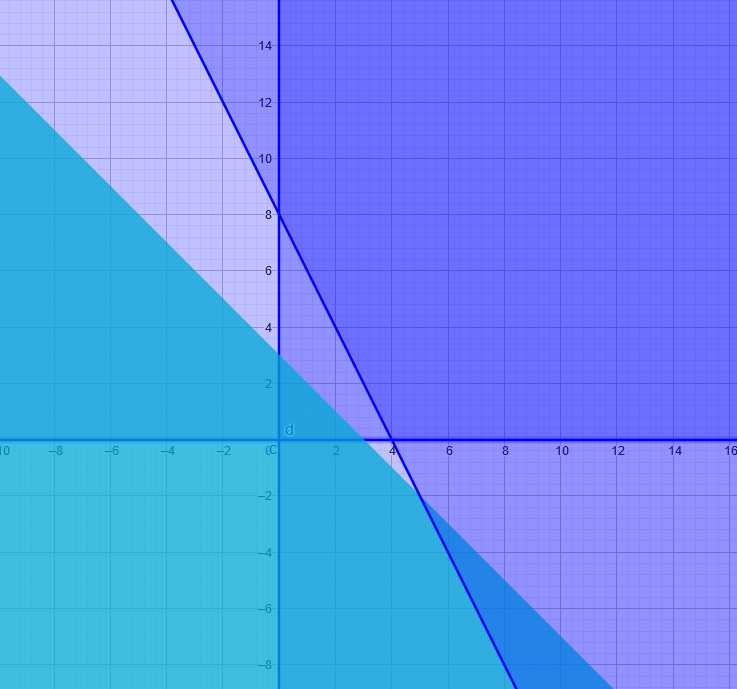
\includegraphics[width=10cm]{pendientes_1_bach/1_sociales/prog_lin.png} \\
    Como no tiene intersección, el sistema no tiene solución
\end{solution}



% \question[10] Una empresa cinematográfica dispone de tres salas A, B y C. Los precios de entrada a cada una de estas salas son 1, 2 y 3\euro \ respectivamente. Un día la recaudación conjunta de las tres salas fue de 425\euro \ y el número total de espectadores que acudieron fue de 200. Si los espectadores de la sala A, hubiesen asistido a la sala B y los de la sala B a la sala A, se obtendría una recaudación de 400\euro. Calcula el número de espectadores que acudió a cada sala.
% \begin{solution}
%     $\left\{ \begin{matrix}x + 2 y + 3 z = 425 \\ x + y + z = 200 \\ 2 x + y + 3 z = 400 \\ \end{matrix}\right.$ \\
%     $A^*=\left(\begin{matrix}1 & 2 & 3 & 425\\1 & 1 & 1 & 200\\2 & 1 & 3 & 400\end{matrix}\right)\sim\left(\begin{matrix}1 & 2 & 3 & 425\\0 & -1 & -2 & -225\\0 & 0 & 3 & 225\end{matrix}\right)\to x=50, y=75, z=75$
% \end{solution}

\question[10] Resuelve las siguientes ecuaciones:
\begin{parts}
    \part $\sqrt {x - 3} {\text{ }} + {\text{ }}\sqrt {{\text{3x - 5}}} {\text{ }} = {\text{ 6}}$
    \begin{solution}
        $x^{2} - 74 x + 469=0 \to [7,67] \to x=7$
    \end{solution}
    % \part $2 \log (x+3) - \log (x-6) = 2$
    % \begin{solution}
    %     $\dfrac{(x+3)^2}{(x-6)}=100 \to x= 7,   x=87$
    % \end{solution}
    % \part $3^{x-1} + 3^{x+2} = 84$
    % \begin{solution}
    %     $3^x(\frac{1}{3}+9)=84 \to 3^x=\frac{84\cdot 3}{28} \to 3^x=9 \to x=2$
    % \end{solution}
    \part $x^5 - 3x^4 - 8x^3 + 12x^2 + 16x = 0$
    \begin{solution}
        $x \left(x - 4\right) \left(x - 2\right) \left(x + 1\right) \left(x + 2\right)=0 \to x=0, x=4, x=2, x=-1, x=-2$
    \end{solution}
\end{parts}
\question[9] Opera, simplifica y racionaliza en todos los casos en que se presente:
\begin{parts}
    \part $\frac{3}{{4\sqrt 2 }}$
    \begin{solution}
        $\frac{3 \sqrt{2}}{8}$
    \end{solution}
    \part $\frac{{\sqrt 6 \, - \,\sqrt 2 }}{{\sqrt {12}  - 2}}$	
    \begin{solution}
        $\dfrac{(\sqrt{6}-\sqrt{2})(2\sqrt{3}+2)}{4\cdot 3 - 4}=\dfrac{\sqrt{2}(\sqrt{3}-1)\cdot 2(\sqrt{3}+1)}{8}=\frac{4\sqrt{2}}{8}=\frac{\sqrt{2}}{2}$
    \end{solution}
    % \part $\sqrt[5]{{{2^2}\sqrt[4]{{8\sqrt[3]{2}}}}}.\sqrt[{30}]{{{2^{43}}}}$
    \part $\sqrt[5]{{{2^2}\sqrt[4]{{8\sqrt[3]{2}}}}}$
    \begin{solution}
        $\sqrt[60]{2^{34}}\cdot \sqrt[60]{2^{86}}=\sqrt[60]{2^{120}}=2^2=4$
    \end{solution}
\end{parts}

\question La cotización en bolsa (en miles de \euro) de los dos valores Minerocat (X) y Construcat (Y) a lo largo de 6 días de sesión son los siguientes:
\begin{center}
\begin{tabular}{|c|c|c|c|c|c|c|}
    \hline
    X= Minerocat & 8 & 7 & 6 & 5 & 7 & 8 \\
    \hline
    Y= Construcat & 6 & 5 & 4.5 & 4 & 4.5 & 5  \\
    \hline
\end{tabular}
   
\end{center}

\begin{parts}
    \part[9] Calcula el coeficiente de correlación de Pearson. Da una interpretación del mismo en términos del enunciado del problema
    \part[6] La cotización en bolsa de Minerocat alcanza el valor 9 un cierto día, ¿qué cotización en bolsa cabe esperar que alcance el valor Construcat?. Es correcta la predicción
\end{parts}
\begin{solution}
\begin{tabular}{lrrrrr}
\hline
        &        a &        b &   $a\cdot b$ &    $a^2$ &   $b^2$ \\
\hline
 0      &  8       &  6       &      48      &  64      &   36    \\
 1      &  7       &  5       &      35      &  49      &   25    \\
 2      &  6       &  4.5     &      27      &  36      &   20.25 \\
 3      &  5       &  4       &      20      &  25      &   16    \\
 4      &  7       &  4.5     &      31.5    &  49      &   20.25 \\
 5      &  8       &  5       &      40      &  64      &   25    \\
 Sumas  & 41       & 29       &     201.5    & 287      &  142.5  \\
 Medias &  6.83333 &  4.83333 &      33.5833 &  47.8333 &   23.75 \\
\hline
\end{tabular}
\\ \\ Las medias son: \\$\overline{a}=\frac{\Sigma{a_i}}{N}=\frac{41.0}{6}=6.83333333333333$. $\overline{b}=\frac{\Sigma{b_i}}{N}=\frac{29.0}{6}=4.83333333333333$.  El centro de gravedad es: $(6.83333333333333,4.83333333333333)$ \\ \\ Varianzas y covarianzas: \\ $\sigma_a=\sqrt{\frac{\sum{a_i^2}}{N}-\overline{a}^2}=\sqrt{\frac{287.0}{6}-6.83333333333333^2}=1.06718737290548$.\\ $\sigma_b=\sqrt{\frac{\sum{b_i^2}}{N}-\overline{b}^2}=\sqrt{\frac{142.5}{6}-4.83333333333333^2}=0.623609564462327$.\\ $\sigma_{ab}=\frac{\sum{a_i \cdot b_i}}{N}-\overline{a}\cdot \overline{b}=\frac{201.5}{6}-6.83333333333333\cdot 4.83333333333333=0.555555555555564$. \\ \\ Correlación: \\ $r=\dfrac{\sigma_{ab}}{\sigma_a \cdot \sigma_b}=\frac{0.555555555555564}{1.06718737290548\cdot 0.623609564462327}=0.83478387112969$. \\ \\ Recta de regresión: \\ La pendiente es: 0.48780487804878, la ordenada en el origen: 1.5, El coeficiente de correlación:0.834783871129682 y la recta de regresión: $y = 0.48780487804878 x + 1.5$
\\

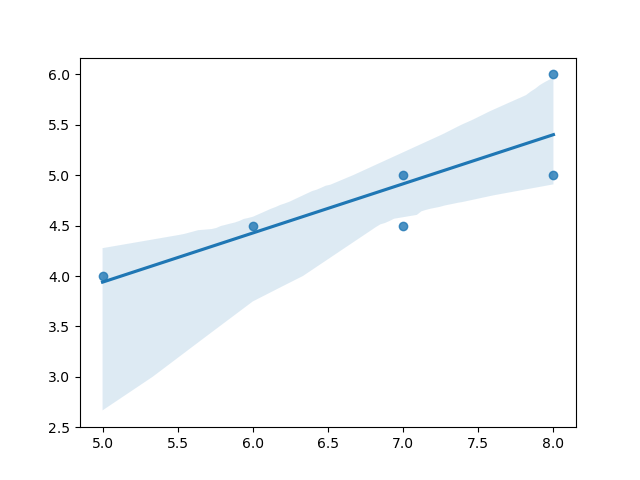
\includegraphics[width=8cm]{pendientes_1_bach/1_sociales/regresion1.png} 
\\

Estimación para $x=9$:
$y=5.89024390243902$

\end{solution}

% \question[10] Dada la función	
% $f(x)=\left\{ \begin{matrix}
%     x & , si \ x >1 \\
%     x^2 & , si \ -1\leq x \leq 1 \\
%     x+2 & , si \ x < -1 \\
%    % \text{   }x\text{  }\text{,  s }\!\!\acute{\mathrm{i}}\!\!\text{    x }>\text{ 1}  \\
%    % \text{  }{{\text{x}}^{\text{2}}}\text{  }\text{,  s }\!\!\acute{\mathrm{i}}\!\!\text{  -1 }\le \text{ x }\le \text{ 1}  \\
%    % \text{x}+\text{2   }\text{,   s }\!\!\acute{\mathrm{i}}\!\!\text{  x }<\text{ -1}  \\
% \end{matrix} \right.$

% Representa dicha función, calculando su dominio, recorrido e intervalos de crecimiento y decrecimiento.
% \begin{solution}
%     \definecolor{ffvvqq}{rgb}{1,0.3333333333333333,0}
% \begin{tikzpicture}[line cap=round,line join=round,>=triangle 45,x=1cm,y=1cm, scale=0.3]
% \begin{axis}[
% x=1cm,y=1cm,
% axis lines=middle,
% ymajorgrids=true,
% xmajorgrids=true,
% xmin=-6.4345028065467655,
% xmax=4.9673889667579285,
% ymin=-4.947174564268295,
% ymax=5.623101302346182,
% xtick={-6,-4,...,4},
% ytick={-4,-2,...,4},]
% \clip(-6.4345028065467655,-4.947174564268295) rectangle (4.9673889667579285,5.623101302346182);
% \draw[line width=2pt,color=ffvvqq] (-6.4345028065467655,-4.4345028065467655) -- (-6.4345028065467655,-4.4345028065467655);
% \draw[line width=2pt,color=ffvvqq] (-6.4345028065467655,-4.4345028065467655) -- (-6.405998077113503,-4.405998077113503);
% \draw[line width=2pt,color=ffvvqq] (-6.405998077113503,-4.405998077113503) -- (-6.377493347680241,-4.377493347680241);
% \draw[line width=2pt,color=ffvvqq] (-6.377493347680241,-4.377493347680241) -- (-6.348988618246979,-4.348988618246979);
% \draw[line width=2pt,color=ffvvqq] (-6.348988618246979,-4.348988618246979) -- (-6.320483888813717,-4.320483888813717);
% \draw[line width=2pt,color=ffvvqq] (-6.320483888813717,-4.320483888813717) -- (-6.291979159380455,-4.291979159380455);
% \draw[line width=2pt,color=ffvvqq] (-6.291979159380455,-4.291979159380455) -- (-6.263474429947193,-4.263474429947193);
% \draw[line width=2pt,color=ffvvqq] (-6.263474429947193,-4.263474429947193) -- (-6.234969700513931,-4.234969700513931);
% \draw[line width=2pt,color=ffvvqq] (-6.234969700513931,-4.234969700513931) -- (-6.206464971080669,-4.206464971080669);
% \draw[line width=2pt,color=ffvvqq] (-6.206464971080669,-4.206464971080669) -- (-6.177960241647407,-4.177960241647407);
% \draw[line width=2pt,color=ffvvqq] (-6.177960241647407,-4.177960241647407) -- (-6.1494555122141445,-4.1494555122141445);
% \draw[line width=2pt,color=ffvvqq] (-6.1494555122141445,-4.1494555122141445) -- (-6.1209507827808824,-4.1209507827808824);
% \draw[line width=2pt,color=ffvvqq] (-6.1209507827808824,-4.1209507827808824) -- (-6.09244605334762,-4.09244605334762);
% \draw[line width=2pt,color=ffvvqq] (-6.09244605334762,-4.09244605334762) -- (-6.063941323914358,-4.063941323914358);
% \draw[line width=2pt,color=ffvvqq] (-6.063941323914358,-4.063941323914358) -- (-6.035436594481096,-4.035436594481096);
% \draw[line width=2pt,color=ffvvqq] (-6.035436594481096,-4.035436594481096) -- (-6.006931865047834,-4.006931865047834);
% \draw[line width=2pt,color=ffvvqq] (-6.006931865047834,-4.006931865047834) -- (-5.978427135614572,-3.978427135614572);
% \draw[line width=2pt,color=ffvvqq] (-5.978427135614572,-3.978427135614572) -- (-5.94992240618131,-3.94992240618131);
% \draw[line width=2pt,color=ffvvqq] (-5.94992240618131,-3.94992240618131) -- (-5.921417676748048,-3.9214176767480478);
% \draw[line width=2pt,color=ffvvqq] (-5.921417676748048,-3.9214176767480478) -- (-5.892912947314786,-3.8929129473147857);
% \draw[line width=2pt,color=ffvvqq] (-5.892912947314786,-3.8929129473147857) -- (-5.8644082178815236,-3.8644082178815236);
% \draw[line width=2pt,color=ffvvqq] (-5.8644082178815236,-3.8644082178815236) -- (-5.8359034884482615,-3.8359034884482615);
% \draw[line width=2pt,color=ffvvqq] (-5.8359034884482615,-3.8359034884482615) -- (-5.807398759014999,-3.8073987590149994);
% \draw[line width=2pt,color=ffvvqq] (-5.807398759014999,-3.8073987590149994) -- (-5.778894029581737,-3.7788940295817373);
% \draw[line width=2pt,color=ffvvqq] (-5.778894029581737,-3.7788940295817373) -- (-5.750389300148475,-3.750389300148475);
% \draw[line width=2pt,color=ffvvqq] (-5.750389300148475,-3.750389300148475) -- (-5.721884570715213,-3.721884570715213);
% \draw[line width=2pt,color=ffvvqq] (-5.721884570715213,-3.721884570715213) -- (-5.693379841281951,-3.693379841281951);
% \draw[line width=2pt,color=ffvvqq] (-5.693379841281951,-3.693379841281951) -- (-5.664875111848689,-3.664875111848689);
% \draw[line width=2pt,color=ffvvqq] (-5.664875111848689,-3.664875111848689) -- (-5.636370382415427,-3.6363703824154268);
% \draw[line width=2pt,color=ffvvqq] (-5.636370382415427,-3.6363703824154268) -- (-5.607865652982165,-3.6078656529821647);
% \draw[line width=2pt,color=ffvvqq] (-5.607865652982165,-3.6078656529821647) -- (-5.579360923548903,-3.5793609235489026);
% \draw[line width=2pt,color=ffvvqq] (-5.579360923548903,-3.5793609235489026) -- (-5.5508561941156405,-3.5508561941156405);
% \draw[line width=2pt,color=ffvvqq] (-5.5508561941156405,-3.5508561941156405) -- (-5.522351464682378,-3.5223514646823784);
% \draw[line width=2pt,color=ffvvqq] (-5.522351464682378,-3.5223514646823784) -- (-5.493846735249116,-3.4938467352491163);
% \draw[line width=2pt,color=ffvvqq] (-5.493846735249116,-3.4938467352491163) -- (-5.465342005815854,-3.465342005815854);
% \draw[line width=2pt,color=ffvvqq] (-5.465342005815854,-3.465342005815854) -- (-5.436837276382592,-3.436837276382592);
% \draw[line width=2pt,color=ffvvqq] (-5.436837276382592,-3.436837276382592) -- (-5.40833254694933,-3.40833254694933);
% \draw[line width=2pt,color=ffvvqq] (-5.40833254694933,-3.40833254694933) -- (-5.379827817516068,-3.379827817516068);
% \draw[line width=2pt,color=ffvvqq] (-5.379827817516068,-3.379827817516068) -- (-5.351323088082806,-3.3513230880828058);
% \draw[line width=2pt,color=ffvvqq] (-5.351323088082806,-3.3513230880828058) -- (-5.322818358649544,-3.3228183586495437);
% \draw[line width=2pt,color=ffvvqq] (-5.322818358649544,-3.3228183586495437) -- (-5.294313629216282,-3.2943136292162816);
% \draw[line width=2pt,color=ffvvqq] (-5.294313629216282,-3.2943136292162816) -- (-5.2658088997830195,-3.2658088997830195);
% \draw[line width=2pt,color=ffvvqq] (-5.2658088997830195,-3.2658088997830195) -- (-5.237304170349757,-3.2373041703497574);
% \draw[line width=2pt,color=ffvvqq] (-5.237304170349757,-3.2373041703497574) -- (-5.208799440916495,-3.2087994409164953);
% \draw[line width=2pt,color=ffvvqq] (-5.208799440916495,-3.2087994409164953) -- (-5.180294711483233,-3.180294711483233);
% \draw[line width=2pt,color=ffvvqq] (-5.180294711483233,-3.180294711483233) -- (-5.151789982049971,-3.151789982049971);
% \draw[line width=2pt,color=ffvvqq] (-5.151789982049971,-3.151789982049971) -- (-5.123285252616709,-3.123285252616709);
% \draw[line width=2pt,color=ffvvqq] (-5.123285252616709,-3.123285252616709) -- (-5.094780523183447,-3.094780523183447);
% \draw[line width=2pt,color=ffvvqq] (-5.094780523183447,-3.094780523183447) -- (-5.066275793750185,-3.0662757937501848);
% \draw[line width=2pt,color=ffvvqq] (-5.066275793750185,-3.0662757937501848) -- (-5.037771064316923,-3.0377710643169227);
% \draw[line width=2pt,color=ffvvqq] (-5.037771064316923,-3.0377710643169227) -- (-5.009266334883661,-3.0092663348836606);
% \draw[line width=2pt,color=ffvvqq] (-5.009266334883661,-3.0092663348836606) -- (-4.9807616054503985,-2.9807616054503985);
% \draw[line width=2pt,color=ffvvqq] (-4.9807616054503985,-2.9807616054503985) -- (-4.952256876017136,-2.9522568760171364);
% \draw[line width=2pt,color=ffvvqq] (-4.952256876017136,-2.9522568760171364) -- (-4.923752146583874,-2.9237521465838743);
% \draw[line width=2pt,color=ffvvqq] (-4.923752146583874,-2.9237521465838743) -- (-4.895247417150612,-2.895247417150612);
% \draw[line width=2pt,color=ffvvqq] (-4.895247417150612,-2.895247417150612) -- (-4.86674268771735,-2.86674268771735);
% \draw[line width=2pt,color=ffvvqq] (-4.86674268771735,-2.86674268771735) -- (-4.838237958284088,-2.838237958284088);
% \draw[line width=2pt,color=ffvvqq] (-4.838237958284088,-2.838237958284088) -- (-4.809733228850826,-2.809733228850826);
% \draw[line width=2pt,color=ffvvqq] (-4.809733228850826,-2.809733228850826) -- (-4.781228499417564,-2.781228499417564);
% \draw[line width=2pt,color=ffvvqq] (-4.781228499417564,-2.781228499417564) -- (-4.752723769984302,-2.7527237699843017);
% \draw[line width=2pt,color=ffvvqq] (-4.752723769984302,-2.7527237699843017) -- (-4.72421904055104,-2.7242190405510396);
% \draw[line width=2pt,color=ffvvqq] (-4.72421904055104,-2.7242190405510396) -- (-4.6957143111177775,-2.6957143111177775);
% \draw[line width=2pt,color=ffvvqq] (-4.6957143111177775,-2.6957143111177775) -- (-4.667209581684515,-2.6672095816845154);
% \draw[line width=2pt,color=ffvvqq] (-4.667209581684515,-2.6672095816845154) -- (-4.638704852251253,-2.6387048522512533);
% \draw[line width=2pt,color=ffvvqq] (-4.638704852251253,-2.6387048522512533) -- (-4.610200122817991,-2.610200122817991);
% \draw[line width=2pt,color=ffvvqq] (-4.610200122817991,-2.610200122817991) -- (-4.581695393384729,-2.581695393384729);
% \draw[line width=2pt,color=ffvvqq] (-4.581695393384729,-2.581695393384729) -- (-4.553190663951467,-2.553190663951467);
% \draw[line width=2pt,color=ffvvqq] (-4.553190663951467,-2.553190663951467) -- (-4.524685934518205,-2.524685934518205);
% \draw[line width=2pt,color=ffvvqq] (-4.524685934518205,-2.524685934518205) -- (-4.496181205084943,-2.496181205084943);
% \draw[line width=2pt,color=ffvvqq] (-4.496181205084943,-2.496181205084943) -- (-4.467676475651681,-2.4676764756516807);
% \draw[line width=2pt,color=ffvvqq] (-4.467676475651681,-2.4676764756516807) -- (-4.439171746218419,-2.4391717462184186);
% \draw[line width=2pt,color=ffvvqq] (-4.439171746218419,-2.4391717462184186) -- (-4.4106670167851565,-2.4106670167851565);
% \draw[line width=2pt,color=ffvvqq] (-4.4106670167851565,-2.4106670167851565) -- (-4.382162287351894,-2.3821622873518944);
% \draw[line width=2pt,color=ffvvqq] (-4.382162287351894,-2.3821622873518944) -- (-4.353657557918632,-2.3536575579186323);
% \draw[line width=2pt,color=ffvvqq] (-4.353657557918632,-2.3536575579186323) -- (-4.32515282848537,-2.32515282848537);
% \draw[line width=2pt,color=ffvvqq] (-4.32515282848537,-2.32515282848537) -- (-4.296648099052108,-2.296648099052108);
% \draw[line width=2pt,color=ffvvqq] (-4.296648099052108,-2.296648099052108) -- (-4.268143369618846,-2.268143369618846);
% \draw[line width=2pt,color=ffvvqq] (-4.268143369618846,-2.268143369618846) -- (-4.239638640185584,-2.239638640185584);
% \draw[line width=2pt,color=ffvvqq] (-4.239638640185584,-2.239638640185584) -- (-4.211133910752322,-2.211133910752322);
% \draw[line width=2pt,color=ffvvqq] (-4.211133910752322,-2.211133910752322) -- (-4.18262918131906,-2.1826291813190597);
% \draw[line width=2pt,color=ffvvqq] (-4.18262918131906,-2.1826291813190597) -- (-4.154124451885798,-2.1541244518857976);
% \draw[line width=2pt,color=ffvvqq] (-4.154124451885798,-2.1541244518857976) -- (-4.1256197224525355,-2.1256197224525355);
% \draw[line width=2pt,color=ffvvqq] (-4.1256197224525355,-2.1256197224525355) -- (-4.097114993019273,-2.0971149930192734);
% \draw[line width=2pt,color=ffvvqq] (-4.097114993019273,-2.0971149930192734) -- (-4.068610263586011,-2.0686102635860113);
% \draw[line width=2pt,color=ffvvqq] (-4.068610263586011,-2.0686102635860113) -- (-4.040105534152749,-2.040105534152749);
% \draw[line width=2pt,color=ffvvqq] (-4.040105534152749,-2.040105534152749) -- (-4.011600804719487,-2.011600804719487);
% \draw[line width=2pt,color=ffvvqq] (-4.011600804719487,-2.011600804719487) -- (-3.9830960752862254,-1.9830960752862254);
% \draw[line width=2pt,color=ffvvqq] (-3.9830960752862254,-1.9830960752862254) -- (-3.954591345852964,-1.9545913458529638);
% \draw[line width=2pt,color=ffvvqq] (-3.954591345852964,-1.9545913458529638) -- (-3.926086616419702,-1.9260866164197021);
% \draw[line width=2pt,color=ffvvqq] (-3.926086616419702,-1.9260866164197021) -- (-3.8975818869864405,-1.8975818869864405);
% \draw[line width=2pt,color=ffvvqq] (-3.8975818869864405,-1.8975818869864405) -- (-3.869077157553179,-1.8690771575531788);
% \draw[line width=2pt,color=ffvvqq] (-3.869077157553179,-1.8690771575531788) -- (-3.840572428119917,-1.8405724281199172);
% \draw[line width=2pt,color=ffvvqq] (-3.840572428119917,-1.8405724281199172) -- (-3.8120676986866555,-1.8120676986866555);
% \draw[line width=2pt,color=ffvvqq] (-3.8120676986866555,-1.8120676986866555) -- (-3.783562969253394,-1.7835629692533939);
% \draw[line width=2pt,color=ffvvqq] (-3.783562969253394,-1.7835629692533939) -- (-3.755058239820132,-1.7550582398201322);
% \draw[line width=2pt,color=ffvvqq] (-3.755058239820132,-1.7550582398201322) -- (-3.7265535103868705,-1.7265535103868705);
% \draw[line width=2pt,color=ffvvqq] (-3.7265535103868705,-1.7265535103868705) -- (-3.698048780953609,-1.698048780953609);
% \draw[line width=2pt,color=ffvvqq] (-3.698048780953609,-1.698048780953609) -- (-3.6695440515203472,-1.6695440515203472);
% \draw[line width=2pt,color=ffvvqq] (-3.6695440515203472,-1.6695440515203472) -- (-3.6410393220870856,-1.6410393220870856);
% \draw[line width=2pt,color=ffvvqq] (-3.6410393220870856,-1.6410393220870856) -- (-3.612534592653824,-1.612534592653824);
% \draw[line width=2pt,color=ffvvqq] (-3.612534592653824,-1.612534592653824) -- (-3.5840298632205623,-1.5840298632205623);
% \draw[line width=2pt,color=ffvvqq] (-3.5840298632205623,-1.5840298632205623) -- (-3.5555251337873006,-1.5555251337873006);
% \draw[line width=2pt,color=ffvvqq] (-3.5555251337873006,-1.5555251337873006) -- (-3.527020404354039,-1.527020404354039);
% \draw[line width=2pt,color=ffvvqq] (-3.527020404354039,-1.527020404354039) -- (-3.4985156749207773,-1.4985156749207773);
% \draw[line width=2pt,color=ffvvqq] (-3.4985156749207773,-1.4985156749207773) -- (-3.4700109454875157,-1.4700109454875157);
% \draw[line width=2pt,color=ffvvqq] (-3.4700109454875157,-1.4700109454875157) -- (-3.441506216054254,-1.441506216054254);
% \draw[line width=2pt,color=ffvvqq] (-3.441506216054254,-1.441506216054254) -- (-3.4130014866209923,-1.4130014866209923);
% \draw[line width=2pt,color=ffvvqq] (-3.4130014866209923,-1.4130014866209923) -- (-3.3844967571877307,-1.3844967571877307);
% \draw[line width=2pt,color=ffvvqq] (-3.3844967571877307,-1.3844967571877307) -- (-3.355992027754469,-1.355992027754469);
% \draw[line width=2pt,color=ffvvqq] (-3.355992027754469,-1.355992027754469) -- (-3.3274872983212074,-1.3274872983212074);
% \draw[line width=2pt,color=ffvvqq] (-3.3274872983212074,-1.3274872983212074) -- (-3.2989825688879457,-1.2989825688879457);
% \draw[line width=2pt,color=ffvvqq] (-3.2989825688879457,-1.2989825688879457) -- (-3.270477839454684,-1.270477839454684);
% \draw[line width=2pt,color=ffvvqq] (-3.270477839454684,-1.270477839454684) -- (-3.2419731100214224,-1.2419731100214224);
% \draw[line width=2pt,color=ffvvqq] (-3.2419731100214224,-1.2419731100214224) -- (-3.2134683805881608,-1.2134683805881608);
% \draw[line width=2pt,color=ffvvqq] (-3.2134683805881608,-1.2134683805881608) -- (-3.184963651154899,-1.184963651154899);
% \draw[line width=2pt,color=ffvvqq] (-3.184963651154899,-1.184963651154899) -- (-3.1564589217216374,-1.1564589217216374);
% \draw[line width=2pt,color=ffvvqq] (-3.1564589217216374,-1.1564589217216374) -- (-3.127954192288376,-1.1279541922883758);
% \draw[line width=2pt,color=ffvvqq] (-3.127954192288376,-1.1279541922883758) -- (-3.099449462855114,-1.0994494628551141);
% \draw[line width=2pt,color=ffvvqq] (-3.099449462855114,-1.0994494628551141) -- (-3.0709447334218525,-1.0709447334218525);
% \draw[line width=2pt,color=ffvvqq] (-3.0709447334218525,-1.0709447334218525) -- (-3.042440003988591,-1.0424400039885908);
% \draw[line width=2pt,color=ffvvqq] (-3.042440003988591,-1.0424400039885908) -- (-3.013935274555329,-1.0139352745553292);
% \draw[line width=2pt,color=ffvvqq] (-3.013935274555329,-1.0139352745553292) -- (-2.9854305451220675,-0.9854305451220675);
% \draw[line width=2pt,color=ffvvqq] (-2.9854305451220675,-0.9854305451220675) -- (-2.956925815688806,-0.9569258156888059);
% \draw[line width=2pt,color=ffvvqq] (-2.956925815688806,-0.9569258156888059) -- (-2.928421086255544,-0.9284210862555442);
% \draw[line width=2pt,color=ffvvqq] (-2.928421086255544,-0.9284210862555442) -- (-2.8999163568222825,-0.8999163568222825);
% \draw[line width=2pt,color=ffvvqq] (-2.8999163568222825,-0.8999163568222825) -- (-2.871411627389021,-0.8714116273890209);
% \draw[line width=2pt,color=ffvvqq] (-2.871411627389021,-0.8714116273890209) -- (-2.8429068979557592,-0.8429068979557592);
% \draw[line width=2pt,color=ffvvqq] (-2.8429068979557592,-0.8429068979557592) -- (-2.8144021685224976,-0.8144021685224976);
% \draw[line width=2pt,color=ffvvqq] (-2.8144021685224976,-0.8144021685224976) -- (-2.785897439089236,-0.7858974390892359);
% \draw[line width=2pt,color=ffvvqq] (-2.785897439089236,-0.7858974390892359) -- (-2.7573927096559743,-0.7573927096559743);
% \draw[line width=2pt,color=ffvvqq] (-2.7573927096559743,-0.7573927096559743) -- (-2.7288879802227126,-0.7288879802227126);
% \draw[line width=2pt,color=ffvvqq] (-2.7288879802227126,-0.7288879802227126) -- (-2.700383250789451,-0.700383250789451);
% \draw[line width=2pt,color=ffvvqq] (-2.700383250789451,-0.700383250789451) -- (-2.6718785213561893,-0.6718785213561893);
% \draw[line width=2pt,color=ffvvqq] (-2.6718785213561893,-0.6718785213561893) -- (-2.6433737919229277,-0.6433737919229277);
% \draw[line width=2pt,color=ffvvqq] (-2.6433737919229277,-0.6433737919229277) -- (-2.614869062489666,-0.614869062489666);
% \draw[line width=2pt,color=ffvvqq] (-2.614869062489666,-0.614869062489666) -- (-2.5863643330564043,-0.5863643330564043);
% \draw[line width=2pt,color=ffvvqq] (-2.5863643330564043,-0.5863643330564043) -- (-2.5578596036231427,-0.5578596036231427);
% \draw[line width=2pt,color=ffvvqq] (-2.5578596036231427,-0.5578596036231427) -- (-2.529354874189881,-0.529354874189881);
% \draw[line width=2pt,color=ffvvqq] (-2.529354874189881,-0.529354874189881) -- (-2.5008501447566194,-0.5008501447566194);
% \draw[line width=2pt,color=ffvvqq] (-2.5008501447566194,-0.5008501447566194) -- (-2.4723454153233577,-0.4723454153233577);
% \draw[line width=2pt,color=ffvvqq] (-2.4723454153233577,-0.4723454153233577) -- (-2.443840685890096,-0.44384068589009606);
% \draw[line width=2pt,color=ffvvqq] (-2.443840685890096,-0.44384068589009606) -- (-2.4153359564568344,-0.4153359564568344);
% \draw[line width=2pt,color=ffvvqq] (-2.4153359564568344,-0.4153359564568344) -- (-2.3868312270235728,-0.38683122702357275);
% \draw[line width=2pt,color=ffvvqq] (-2.3868312270235728,-0.38683122702357275) -- (-2.358326497590311,-0.3583264975903111);
% \draw[line width=2pt,color=ffvvqq] (-2.358326497590311,-0.3583264975903111) -- (-2.3298217681570494,-0.32982176815704944);
% \draw[line width=2pt,color=ffvvqq] (-2.3298217681570494,-0.32982176815704944) -- (-2.301317038723788,-0.3013170387237878);
% \draw[line width=2pt,color=ffvvqq] (-2.301317038723788,-0.3013170387237878) -- (-2.272812309290526,-0.27281230929052613);
% \draw[line width=2pt,color=ffvvqq] (-2.272812309290526,-0.27281230929052613) -- (-2.2443075798572645,-0.24430757985726448);
% \draw[line width=2pt,color=ffvvqq] (-2.2443075798572645,-0.24430757985726448) -- (-2.215802850424003,-0.21580285042400282);
% \draw[line width=2pt,color=ffvvqq] (-2.215802850424003,-0.21580285042400282) -- (-2.187298120990741,-0.18729812099074117);
% \draw[line width=2pt,color=ffvvqq] (-2.187298120990741,-0.18729812099074117) -- (-2.1587933915574795,-0.1587933915574795);
% \draw[line width=2pt,color=ffvvqq] (-2.1587933915574795,-0.1587933915574795) -- (-2.130288662124218,-0.13028866212421786);
% \draw[line width=2pt,color=ffvvqq] (-2.130288662124218,-0.13028866212421786) -- (-2.101783932690956,-0.1017839326909562);
% \draw[line width=2pt,color=ffvvqq] (-2.101783932690956,-0.1017839326909562) -- (-2.0732792032576945,-0.07327920325769455);
% \draw[line width=2pt,color=ffvvqq] (-2.0732792032576945,-0.07327920325769455) -- (-2.044774473824433,-0.04477447382443289);
% \draw[line width=2pt,color=ffvvqq] (-2.044774473824433,-0.04477447382443289) -- (-2.0162697443911712,-0.016269744391171237);
% \draw[line width=2pt,color=ffvvqq] (-2.0162697443911712,-0.016269744391171237) -- (-1.9877650149579096,0.012234985042090418);
% \draw[line width=2pt,color=ffvvqq] (-1.9877650149579096,0.012234985042090418) -- (-1.959260285524648,0.04073971447535207);
% \draw[line width=2pt,color=ffvvqq] (-1.959260285524648,0.04073971447535207) -- (-1.9307555560913863,0.06924444390861373);
% \draw[line width=2pt,color=ffvvqq] (-1.9307555560913863,0.06924444390861373) -- (-1.9022508266581246,0.09774917334187538);
% \draw[line width=2pt,color=ffvvqq] (-1.9022508266581246,0.09774917334187538) -- (-1.873746097224863,0.12625390277513704);
% \draw[line width=2pt,color=ffvvqq] (-1.873746097224863,0.12625390277513704) -- (-1.8452413677916013,0.1547586322083987);
% \draw[line width=2pt,color=ffvvqq] (-1.8452413677916013,0.1547586322083987) -- (-1.8167366383583397,0.18326336164166035);
% \draw[line width=2pt,color=ffvvqq] (-1.8167366383583397,0.18326336164166035) -- (-1.788231908925078,0.211768091074922);
% \draw[line width=2pt,color=ffvvqq] (-1.788231908925078,0.211768091074922) -- (-1.7597271794918163,0.24027282050818366);
% \draw[line width=2pt,color=ffvvqq] (-1.7597271794918163,0.24027282050818366) -- (-1.7312224500585547,0.2687775499414453);
% \draw[line width=2pt,color=ffvvqq] (-1.7312224500585547,0.2687775499414453) -- (-1.702717720625293,0.29728227937470697);
% \draw[line width=2pt,color=ffvvqq] (-1.702717720625293,0.29728227937470697) -- (-1.6742129911920314,0.3257870088079686);
% \draw[line width=2pt,color=ffvvqq] (-1.6742129911920314,0.3257870088079686) -- (-1.6457082617587697,0.3542917382412303);
% \draw[line width=2pt,color=ffvvqq] (-1.6457082617587697,0.3542917382412303) -- (-1.617203532325508,0.38279646767449194);
% \draw[line width=2pt,color=ffvvqq] (-1.617203532325508,0.38279646767449194) -- (-1.5886988028922464,0.4113011971077536);
% \draw[line width=2pt,color=ffvvqq] (-1.5886988028922464,0.4113011971077536) -- (-1.5601940734589848,0.43980592654101525);
% \draw[line width=2pt,color=ffvvqq] (-1.5601940734589848,0.43980592654101525) -- (-1.531689344025723,0.4683106559742769);
% \draw[line width=2pt,color=ffvvqq] (-1.531689344025723,0.4683106559742769) -- (-1.5031846145924614,0.49681538540753856);
% \draw[line width=2pt,color=ffvvqq] (-1.5031846145924614,0.49681538540753856) -- (-1.4746798851591998,0.5253201148408002);
% \draw[line width=2pt,color=ffvvqq] (-1.4746798851591998,0.5253201148408002) -- (-1.4461751557259381,0.5538248442740619);
% \draw[line width=2pt,color=ffvvqq] (-1.4461751557259381,0.5538248442740619) -- (-1.4176704262926765,0.5823295737073235);
% \draw[line width=2pt,color=ffvvqq] (-1.4176704262926765,0.5823295737073235) -- (-1.3891656968594148,0.6108343031405852);
% \draw[line width=2pt,color=ffvvqq] (-1.3891656968594148,0.6108343031405852) -- (-1.3606609674261532,0.6393390325738468);
% \draw[line width=2pt,color=ffvvqq] (-1.3606609674261532,0.6393390325738468) -- (-1.3321562379928915,0.6678437620071085);
% \draw[line width=2pt,color=ffvvqq] (-1.3321562379928915,0.6678437620071085) -- (-1.3036515085596299,0.6963484914403701);
% \draw[line width=2pt,color=ffvvqq] (-1.3036515085596299,0.6963484914403701) -- (-1.2751467791263682,0.7248532208736318);
% \draw[line width=2pt,color=ffvvqq] (-1.2751467791263682,0.7248532208736318) -- (-1.2466420496931065,0.7533579503068935);
% \draw[line width=2pt,color=ffvvqq] (-1.2466420496931065,0.7533579503068935) -- (-1.218137320259845,0.7818626797401551);
% \draw[line width=2pt,color=ffvvqq] (-1.218137320259845,0.7818626797401551) -- (-1.1896325908265832,0.8103674091734168);
% \draw[line width=2pt,color=ffvvqq] (-1.1896325908265832,0.8103674091734168) -- (-1.1611278613933216,0.8388721386066784);
% \draw[line width=2pt,color=ffvvqq] (-1.1611278613933216,0.8388721386066784) -- (-1.13262313196006,0.8673768680399401);
% \draw[line width=2pt,color=ffvvqq] (-1.13262313196006,0.8673768680399401) -- (-1.1041184025267983,0.8958815974732017);
% \draw[line width=2pt,color=ffvvqq] (-1.1041184025267983,0.8958815974732017) -- (-1.0756136730935366,0.9243863269064634);
% \draw[line width=2pt,color=ffvvqq] (-1.0756136730935366,0.9243863269064634) -- (-1.047108943660275,0.952891056339725);
% \draw[line width=2pt,color=ffvvqq] (-1.047108943660275,0.952891056339725) -- (-1.0186042142270133,0.9813957857729867);
% \draw[line width=2pt,color=ffvvqq] (-1.0186042142270133,0.9813957857729867) -- (-0.9900994847937515,0.9802969897888523);
% \draw[line width=2pt,color=ffvvqq] (-0.9900994847937515,0.9802969897888523) -- (-0.9615947553604898,0.9246644735368001);
% \draw[line width=2pt,color=ffvvqq] (-0.9615947553604898,0.9246644735368001) -- (-0.933090025927228,0.870656996484875);
% \draw[line width=2pt,color=ffvvqq] (-0.933090025927228,0.870656996484875) -- (-0.9045852964939662,0.8182745586330769);
% \draw[line width=2pt,color=ffvvqq] (-0.9045852964939662,0.8182745586330769) -- (-0.8760805670607045,0.7675171599814055);
% \draw[line width=2pt,color=ffvvqq] (-0.8760805670607045,0.7675171599814055) -- (-0.8475758376274427,0.7183848005298611);
% \draw[line width=2pt,color=ffvvqq] (-0.8475758376274427,0.7183848005298611) -- (-0.8190711081941809,0.6708774802784436);
% \draw[line width=2pt,color=ffvvqq] (-0.8190711081941809,0.6708774802784436) -- (-0.7905663787609192,0.6249951992271531);
% \draw[line width=2pt,color=ffvvqq] (-0.7905663787609192,0.6249951992271531) -- (-0.7620616493276574,0.5807379573759895);
% \draw[line width=2pt,color=ffvvqq] (-0.7620616493276574,0.5807379573759895) -- (-0.7335569198943956,0.5381057547249528);
% \draw[line width=2pt,color=ffvvqq] (-0.7335569198943956,0.5381057547249528) -- (-0.7050521904611339,0.497098591274043);
% \draw[line width=2pt,color=ffvvqq] (-0.7050521904611339,0.497098591274043) -- (-0.6765474610278721,0.45771646702326013);
% \draw[line width=2pt,color=ffvvqq] (-0.6765474610278721,0.45771646702326013) -- (-0.6480427315946103,0.4199593819726042);
% \draw[line width=2pt,color=ffvvqq] (-0.6480427315946103,0.4199593819726042) -- (-0.6195380021613486,0.38382733612207515);
% \draw[line width=2pt,color=ffvvqq] (-0.6195380021613486,0.38382733612207515) -- (-0.5910332727280868,0.349320329471673);
% \draw[line width=2pt,color=ffvvqq] (-0.5910332727280868,0.349320329471673) -- (-0.562528543294825,0.31643836202139786);
% \draw[line width=2pt,color=ffvvqq] (-0.562528543294825,0.31643836202139786) -- (-0.5340238138615633,0.2851814337712496);
% \draw[line width=2pt,color=ffvvqq] (-0.5340238138615633,0.2851814337712496) -- (-0.5055190844283015,0.2555495447212282);
% \draw[line width=2pt,color=ffvvqq] (-0.5055190844283015,0.2555495447212282) -- (-0.4770143549950398,0.22754269487133386);
% \draw[line width=2pt,color=ffvvqq] (-0.4770143549950398,0.22754269487133386) -- (-0.4485096255617781,0.2011608842215664);
% \draw[line width=2pt,color=ffvvqq] (-0.4485096255617781,0.2011608842215664) -- (-0.4200048961285164,0.17640411277192583);
% \draw[line width=2pt,color=ffvvqq] (-0.4200048961285164,0.17640411277192583) -- (-0.39150016669525467,0.15327238052241218);
% \draw[line width=2pt,color=ffvvqq] (-0.39150016669525467,0.15327238052241218) -- (-0.36299543726199296,0.13176568747302547);
% \draw[line width=2pt,color=ffvvqq] (-0.36299543726199296,0.13176568747302547) -- (-0.33449070782873125,0.11188403362376566);
% \draw[line width=2pt,color=ffvvqq] (-0.33449070782873125,0.11188403362376566) -- (-0.30598597839546954,0.09362741897463275);
% \draw[line width=2pt,color=ffvvqq] (-0.30598597839546954,0.09362741897463275) -- (-0.2774812489622078,0.07699584352562676);
% \draw[line width=2pt,color=ffvvqq] (-0.2774812489622078,0.07699584352562676) -- (-0.2489765195289461,0.061989307276747674);
% \draw[line width=2pt,color=ffvvqq] (-0.2489765195289461,0.061989307276747674) -- (-0.22047179009568435,0.0486078102279955);
% \draw[line width=2pt,color=ffvvqq] (-0.22047179009568435,0.0486078102279955) -- (-0.1919670606624226,0.03685135237937024);
% \draw[line width=2pt,color=ffvvqq] (-0.1919670606624226,0.03685135237937024) -- (-0.16346233122916087,0.026719933730871902);
% \draw[line width=2pt,color=ffvvqq] (-0.16346233122916087,0.026719933730871902) -- (-0.13495760179589913,0.018213554282500478);
% \draw[line width=2pt,color=ffvvqq] (-0.13495760179589913,0.018213554282500478) -- (-0.1064528723626374,0.011332214034255968);
% \draw[line width=2pt,color=ffvvqq] (-0.1064528723626374,0.011332214034255968) -- (-0.07794814292937566,0.006075912986138376);
% \draw[line width=2pt,color=ffvvqq] (-0.07794814292937566,0.006075912986138376) -- (-0.04944341349611392,0.0024446511381477003);
% \draw[line width=2pt,color=ffvvqq] (-0.04944341349611392,0.0024446511381477003) -- (-0.020938684062852184,0);
% \draw[line width=2pt,color=ffvvqq] (-0.020938684062852184,0) -- (0.007566045370409551,0);
% \draw[line width=2pt,color=ffvvqq] (0.007566045370409551,0) -- (0.03607077480367128,0.001301100794937167);
% \draw[line width=2pt,color=ffvvqq] (0.03607077480367128,0.001301100794937167) -- (0.06457550423693302,0.004169995747454154);
% \draw[line width=2pt,color=ffvvqq] (0.06457550423693302,0.004169995747454154) -- (0.09308023367019476,0.008663929900098058);
% \draw[line width=2pt,color=ffvvqq] (0.09308023367019476,0.008663929900098058) -- (0.1215849631034565,0.014782903252868879);
% \draw[line width=2pt,color=ffvvqq] (0.1215849631034565,0.014782903252868879) -- (0.15008969253671822,0.02252691580576661);
% \draw[line width=2pt,color=ffvvqq] (0.15008969253671822,0.02252691580576661) -- (0.17859442196997996,0.03189596755879126);
% \draw[line width=2pt,color=ffvvqq] (0.17859442196997996,0.03189596755879126) -- (0.2070991514032417,0.04289005851194283);
% \draw[line width=2pt,color=ffvvqq] (0.2070991514032417,0.04289005851194283) -- (0.23560388083650344,0.05550918866522131);
% \draw[line width=2pt,color=ffvvqq] (0.23560388083650344,0.05550918866522131) -- (0.2641086102697652,0.06975335801862671);
% \draw[line width=2pt,color=ffvvqq] (0.2641086102697652,0.06975335801862671) -- (0.2926133397030269,0.08562256657215901);
% \draw[line width=2pt,color=ffvvqq] (0.2926133397030269,0.08562256657215901) -- (0.3211180691362886,0.10311681432581822);
% \draw[line width=2pt,color=ffvvqq] (0.3211180691362886,0.10311681432581822) -- (0.3496227985695503,0.12223610127960435);
% \draw[line width=2pt,color=ffvvqq] (0.3496227985695503,0.12223610127960435) -- (0.378127528002812,0.14298042743351738);
% \draw[line width=2pt,color=ffvvqq] (0.378127528002812,0.14298042743351738) -- (0.40663225743607373,0.16534979278755735);
% \draw[line width=2pt,color=ffvvqq] (0.40663225743607373,0.16534979278755735) -- (0.43513698686933544,0.1893441973417242);
% \draw[line width=2pt,color=ffvvqq] (0.43513698686933544,0.1893441973417242) -- (0.46364171630259715,0.21496364109601798);
% \draw[line width=2pt,color=ffvvqq] (0.46364171630259715,0.21496364109601798) -- (0.49214644573585886,0.24220812405043868);
% \draw[line width=2pt,color=ffvvqq] (0.49214644573585886,0.24220812405043868) -- (0.5206511751691206,0.2710776462049863);
% \draw[line width=2pt,color=ffvvqq] (0.5206511751691206,0.2710776462049863) -- (0.5491559046023824,0.3015722075596609);
% \draw[line width=2pt,color=ffvvqq] (0.5491559046023824,0.3015722075596609) -- (0.5776606340356442,0.3336918081144624);
% \draw[line width=2pt,color=ffvvqq] (0.5776606340356442,0.3336918081144624) -- (0.6061653634689059,0.36743644786939084);
% \draw[line width=2pt,color=ffvvqq] (0.6061653634689059,0.36743644786939084) -- (0.6346700929021677,0.40280612682444616);
% \draw[line width=2pt,color=ffvvqq] (0.6346700929021677,0.40280612682444616) -- (0.6631748223354295,0.4398008449796284);
% \draw[line width=2pt,color=ffvvqq] (0.6631748223354295,0.4398008449796284) -- (0.6916795517686912,0.4784206023349376);
% \draw[line width=2pt,color=ffvvqq] (0.6916795517686912,0.4784206023349376) -- (0.720184281201953,0.5186653988903737);
% \draw[line width=2pt,color=ffvvqq] (0.720184281201953,0.5186653988903737) -- (0.7486890106352148,0.5605352346459367);
% \draw[line width=2pt,color=ffvvqq] (0.7486890106352148,0.5605352346459367) -- (0.7771937400684765,0.6040301096016266);
% \draw[line width=2pt,color=ffvvqq] (0.7771937400684765,0.6040301096016266) -- (0.8056984695017383,0.6491500237574435);
% \draw[line width=2pt,color=ffvvqq] (0.8056984695017383,0.6491500237574435) -- (0.8342031989350001,0.6958949771133873);
% \draw[line width=2pt,color=ffvvqq] (0.8342031989350001,0.6958949771133873) -- (0.8627079283682618,0.744264969669458);
% \draw[line width=2pt,color=ffvvqq] (0.8627079283682618,0.744264969669458) -- (0.8912126578015236,0.7942600014256556);
% \draw[line width=2pt,color=ffvvqq] (0.8912126578015236,0.7942600014256556) -- (0.9197173872347854,0.8458800723819802);
% \draw[line width=2pt,color=ffvvqq] (0.9197173872347854,0.8458800723819802) -- (0.9482221166680471,0.8991251825384315);
% \draw[line width=2pt,color=ffvvqq] (0.9482221166680471,0.8991251825384315) -- (0.9767268461013089,0.95399533189501);
% \draw[line width=2pt,color=ffvvqq] (0.9767268461013089,0.95399533189501) -- (1.0052315755345707,1.0052315755345707);
% \draw[line width=2pt,color=ffvvqq] (1.0052315755345707,1.0052315755345707) -- (1.0337363049678323,1.0337363049678323);
% \draw[line width=2pt,color=ffvvqq] (1.0337363049678323,1.0337363049678323) -- (1.062241034401094,1.062241034401094);
% \draw[line width=2pt,color=ffvvqq] (1.062241034401094,1.062241034401094) -- (1.0907457638343556,1.0907457638343556);
% \draw[line width=2pt,color=ffvvqq] (1.0907457638343556,1.0907457638343556) -- (1.1192504932676173,1.1192504932676173);
% \draw[line width=2pt,color=ffvvqq] (1.1192504932676173,1.1192504932676173) -- (1.147755222700879,1.147755222700879);
% \draw[line width=2pt,color=ffvvqq] (1.147755222700879,1.147755222700879) -- (1.1762599521341406,1.1762599521341406);
% \draw[line width=2pt,color=ffvvqq] (1.1762599521341406,1.1762599521341406) -- (1.2047646815674022,1.2047646815674022);
% \draw[line width=2pt,color=ffvvqq] (1.2047646815674022,1.2047646815674022) -- (1.233269411000664,1.233269411000664);
% \draw[line width=2pt,color=ffvvqq] (1.233269411000664,1.233269411000664) -- (1.2617741404339256,1.2617741404339256);
% \draw[line width=2pt,color=ffvvqq] (1.2617741404339256,1.2617741404339256) -- (1.2902788698671872,1.2902788698671872);
% \draw[line width=2pt,color=ffvvqq] (1.2902788698671872,1.2902788698671872) -- (1.3187835993004489,1.3187835993004489);
% \draw[line width=2pt,color=ffvvqq] (1.3187835993004489,1.3187835993004489) -- (1.3472883287337105,1.3472883287337105);
% \draw[line width=2pt,color=ffvvqq] (1.3472883287337105,1.3472883287337105) -- (1.3757930581669722,1.3757930581669722);
% \draw[line width=2pt,color=ffvvqq] (1.3757930581669722,1.3757930581669722) -- (1.4042977876002338,1.4042977876002338);
% \draw[line width=2pt,color=ffvvqq] (1.4042977876002338,1.4042977876002338) -- (1.4328025170334955,1.4328025170334955);
% \draw[line width=2pt,color=ffvvqq] (1.4328025170334955,1.4328025170334955) -- (1.4613072464667571,1.4613072464667571);
% \draw[line width=2pt,color=ffvvqq] (1.4613072464667571,1.4613072464667571) -- (1.4898119759000188,1.4898119759000188);
% \draw[line width=2pt,color=ffvvqq] (1.4898119759000188,1.4898119759000188) -- (1.5183167053332804,1.5183167053332804);
% \draw[line width=2pt,color=ffvvqq] (1.5183167053332804,1.5183167053332804) -- (1.546821434766542,1.546821434766542);
% \draw[line width=2pt,color=ffvvqq] (1.546821434766542,1.546821434766542) -- (1.5753261641998038,1.5753261641998038);
% \draw[line width=2pt,color=ffvvqq] (1.5753261641998038,1.5753261641998038) -- (1.6038308936330654,1.6038308936330654);
% \draw[line width=2pt,color=ffvvqq] (1.6038308936330654,1.6038308936330654) -- (1.632335623066327,1.632335623066327);
% \draw[line width=2pt,color=ffvvqq] (1.632335623066327,1.632335623066327) -- (1.6608403524995887,1.6608403524995887);
% \draw[line width=2pt,color=ffvvqq] (1.6608403524995887,1.6608403524995887) -- (1.6893450819328504,1.6893450819328504);
% \draw[line width=2pt,color=ffvvqq] (1.6893450819328504,1.6893450819328504) -- (1.717849811366112,1.717849811366112);
% \draw[line width=2pt,color=ffvvqq] (1.717849811366112,1.717849811366112) -- (1.7463545407993737,1.7463545407993737);
% \draw[line width=2pt,color=ffvvqq] (1.7463545407993737,1.7463545407993737) -- (1.7748592702326353,1.7748592702326353);
% \draw[line width=2pt,color=ffvvqq] (1.7748592702326353,1.7748592702326353) -- (1.803363999665897,1.803363999665897);
% \draw[line width=2pt,color=ffvvqq] (1.803363999665897,1.803363999665897) -- (1.8318687290991587,1.8318687290991587);
% \draw[line width=2pt,color=ffvvqq] (1.8318687290991587,1.8318687290991587) -- (1.8603734585324203,1.8603734585324203);
% \draw[line width=2pt,color=ffvvqq] (1.8603734585324203,1.8603734585324203) -- (1.888878187965682,1.888878187965682);
% \draw[line width=2pt,color=ffvvqq] (1.888878187965682,1.888878187965682) -- (1.9173829173989436,1.9173829173989436);
% \draw[line width=2pt,color=ffvvqq] (1.9173829173989436,1.9173829173989436) -- (1.9458876468322053,1.9458876468322053);
% \draw[line width=2pt,color=ffvvqq] (1.9458876468322053,1.9458876468322053) -- (1.974392376265467,1.974392376265467);
% \draw[line width=2pt,color=ffvvqq] (1.974392376265467,1.974392376265467) -- (2.002897105698729,2.002897105698729);
% \draw[line width=2pt,color=ffvvqq] (2.002897105698729,2.002897105698729) -- (2.0314018351319905,2.0314018351319905);
% \draw[line width=2pt,color=ffvvqq] (2.0314018351319905,2.0314018351319905) -- (2.059906564565252,2.059906564565252);
% \draw[line width=2pt,color=ffvvqq] (2.059906564565252,2.059906564565252) -- (2.0884112939985138,2.0884112939985138);
% \draw[line width=2pt,color=ffvvqq] (2.0884112939985138,2.0884112939985138) -- (2.1169160234317754,2.1169160234317754);
% \draw[line width=2pt,color=ffvvqq] (2.1169160234317754,2.1169160234317754) -- (2.145420752865037,2.145420752865037);
% \draw[line width=2pt,color=ffvvqq] (2.145420752865037,2.145420752865037) -- (2.1739254822982987,2.1739254822982987);
% \draw[line width=2pt,color=ffvvqq] (2.1739254822982987,2.1739254822982987) -- (2.2024302117315604,2.2024302117315604);
% \draw[line width=2pt,color=ffvvqq] (2.2024302117315604,2.2024302117315604) -- (2.230934941164822,2.230934941164822);
% \draw[line width=2pt,color=ffvvqq] (2.230934941164822,2.230934941164822) -- (2.2594396705980837,2.2594396705980837);
% \draw[line width=2pt,color=ffvvqq] (2.2594396705980837,2.2594396705980837) -- (2.2879444000313454,2.2879444000313454);
% \draw[line width=2pt,color=ffvvqq] (2.2879444000313454,2.2879444000313454) -- (2.316449129464607,2.316449129464607);
% \draw[line width=2pt,color=ffvvqq] (2.316449129464607,2.316449129464607) -- (2.3449538588978687,2.3449538588978687);
% \draw[line width=2pt,color=ffvvqq] (2.3449538588978687,2.3449538588978687) -- (2.3734585883311303,2.3734585883311303);
% \draw[line width=2pt,color=ffvvqq] (2.3734585883311303,2.3734585883311303) -- (2.401963317764392,2.401963317764392);
% \draw[line width=2pt,color=ffvvqq] (2.401963317764392,2.401963317764392) -- (2.4304680471976536,2.4304680471976536);
% \draw[line width=2pt,color=ffvvqq] (2.4304680471976536,2.4304680471976536) -- (2.4589727766309153,2.4589727766309153);
% \draw[line width=2pt,color=ffvvqq] (2.4589727766309153,2.4589727766309153) -- (2.487477506064177,2.487477506064177);
% \draw[line width=2pt,color=ffvvqq] (2.487477506064177,2.487477506064177) -- (2.5159822354974386,2.5159822354974386);
% \draw[line width=2pt,color=ffvvqq] (2.5159822354974386,2.5159822354974386) -- (2.5444869649307003,2.5444869649307003);
% \draw[line width=2pt,color=ffvvqq] (2.5444869649307003,2.5444869649307003) -- (2.572991694363962,2.572991694363962);
% \draw[line width=2pt,color=ffvvqq] (2.572991694363962,2.572991694363962) -- (2.6014964237972236,2.6014964237972236);
% \draw[line width=2pt,color=ffvvqq] (2.6014964237972236,2.6014964237972236) -- (2.6300011532304852,2.6300011532304852);
% \draw[line width=2pt,color=ffvvqq] (2.6300011532304852,2.6300011532304852) -- (2.658505882663747,2.658505882663747);
% \draw[line width=2pt,color=ffvvqq] (2.658505882663747,2.658505882663747) -- (2.6870106120970085,2.6870106120970085);
% \draw[line width=2pt,color=ffvvqq] (2.6870106120970085,2.6870106120970085) -- (2.71551534153027,2.71551534153027);
% \draw[line width=2pt,color=ffvvqq] (2.71551534153027,2.71551534153027) -- (2.744020070963532,2.744020070963532);
% \draw[line width=2pt,color=ffvvqq] (2.744020070963532,2.744020070963532) -- (2.7725248003967935,2.7725248003967935);
% \draw[line width=2pt,color=ffvvqq] (2.7725248003967935,2.7725248003967935) -- (2.801029529830055,2.801029529830055);
% \draw[line width=2pt,color=ffvvqq] (2.801029529830055,2.801029529830055) -- (2.829534259263317,2.829534259263317);
% \draw[line width=2pt,color=ffvvqq] (2.829534259263317,2.829534259263317) -- (2.8580389886965785,2.8580389886965785);
% \draw[line width=2pt,color=ffvvqq] (2.8580389886965785,2.8580389886965785) -- (2.88654371812984,2.88654371812984);
% \draw[line width=2pt,color=ffvvqq] (2.88654371812984,2.88654371812984) -- (2.9150484475631018,2.9150484475631018);
% \draw[line width=2pt,color=ffvvqq] (2.9150484475631018,2.9150484475631018) -- (2.9435531769963634,2.9435531769963634);
% \draw[line width=2pt,color=ffvvqq] (2.9435531769963634,2.9435531769963634) -- (2.972057906429625,2.972057906429625);
% \draw[line width=2pt,color=ffvvqq] (2.972057906429625,2.972057906429625) -- (3.0005626358628867,3.0005626358628867);
% \draw[line width=2pt,color=ffvvqq] (3.0005626358628867,3.0005626358628867) -- (3.0290673652961484,3.0290673652961484);
% \draw[line width=2pt,color=ffvvqq] (3.0290673652961484,3.0290673652961484) -- (3.05757209472941,3.05757209472941);
% \draw[line width=2pt,color=ffvvqq] (3.05757209472941,3.05757209472941) -- (3.0860768241626717,3.0860768241626717);
% \draw[line width=2pt,color=ffvvqq] (3.0860768241626717,3.0860768241626717) -- (3.1145815535959334,3.1145815535959334);
% \draw[line width=2pt,color=ffvvqq] (3.1145815535959334,3.1145815535959334) -- (3.143086283029195,3.143086283029195);
% \draw[line width=2pt,color=ffvvqq] (3.143086283029195,3.143086283029195) -- (3.1715910124624567,3.1715910124624567);
% \draw[line width=2pt,color=ffvvqq] (3.1715910124624567,3.1715910124624567) -- (3.2000957418957183,3.2000957418957183);
% \draw[line width=2pt,color=ffvvqq] (3.2000957418957183,3.2000957418957183) -- (3.22860047132898,3.22860047132898);
% \draw[line width=2pt,color=ffvvqq] (3.22860047132898,3.22860047132898) -- (3.2571052007622416,3.2571052007622416);
% \draw[line width=2pt,color=ffvvqq] (3.2571052007622416,3.2571052007622416) -- (3.2856099301955033,3.2856099301955033);
% \draw[line width=2pt,color=ffvvqq] (3.2856099301955033,3.2856099301955033) -- (3.314114659628765,3.314114659628765);
% \draw[line width=2pt,color=ffvvqq] (3.314114659628765,3.314114659628765) -- (3.3426193890620266,3.3426193890620266);
% \draw[line width=2pt,color=ffvvqq] (3.3426193890620266,3.3426193890620266) -- (3.3711241184952883,3.3711241184952883);
% \draw[line width=2pt,color=ffvvqq] (3.3711241184952883,3.3711241184952883) -- (3.39962884792855,3.39962884792855);
% \draw[line width=2pt,color=ffvvqq] (3.39962884792855,3.39962884792855) -- (3.4281335773618116,3.4281335773618116);
% \draw[line width=2pt,color=ffvvqq] (3.4281335773618116,3.4281335773618116) -- (3.4566383067950732,3.4566383067950732);
% \draw[line width=2pt,color=ffvvqq] (3.4566383067950732,3.4566383067950732) -- (3.485143036228335,3.485143036228335);
% \draw[line width=2pt,color=ffvvqq] (3.485143036228335,3.485143036228335) -- (3.5136477656615965,3.5136477656615965);
% \draw[line width=2pt,color=ffvvqq] (3.5136477656615965,3.5136477656615965) -- (3.542152495094858,3.542152495094858);
% \draw[line width=2pt,color=ffvvqq] (3.542152495094858,3.542152495094858) -- (3.57065722452812,3.57065722452812);
% \draw[line width=2pt,color=ffvvqq] (3.57065722452812,3.57065722452812) -- (3.5991619539613815,3.5991619539613815);
% \draw[line width=2pt,color=ffvvqq] (3.5991619539613815,3.5991619539613815) -- (3.627666683394643,3.627666683394643);
% \draw[line width=2pt,color=ffvvqq] (3.627666683394643,3.627666683394643) -- (3.656171412827905,3.656171412827905);
% \draw[line width=2pt,color=ffvvqq] (3.656171412827905,3.656171412827905) -- (3.6846761422611665,3.6846761422611665);
% \draw[line width=2pt,color=ffvvqq] (3.6846761422611665,3.6846761422611665) -- (3.713180871694428,3.713180871694428);
% \draw[line width=2pt,color=ffvvqq] (3.713180871694428,3.713180871694428) -- (3.7416856011276898,3.7416856011276898);
% \draw[line width=2pt,color=ffvvqq] (3.7416856011276898,3.7416856011276898) -- (3.7701903305609514,3.7701903305609514);
% \draw[line width=2pt,color=ffvvqq] (3.7701903305609514,3.7701903305609514) -- (3.798695059994213,3.798695059994213);
% \draw[line width=2pt,color=ffvvqq] (3.798695059994213,3.798695059994213) -- (3.8271997894274747,3.8271997894274747);
% \draw[line width=2pt,color=ffvvqq] (3.8271997894274747,3.8271997894274747) -- (3.8557045188607364,3.8557045188607364);
% \draw[line width=2pt,color=ffvvqq] (3.8557045188607364,3.8557045188607364) -- (3.884209248293998,3.884209248293998);
% \draw[line width=2pt,color=ffvvqq] (3.884209248293998,3.884209248293998) -- (3.9127139777272597,3.9127139777272597);
% \draw[line width=2pt,color=ffvvqq] (3.9127139777272597,3.9127139777272597) -- (3.9412187071605214,3.9412187071605214);
% \draw[line width=2pt,color=ffvvqq] (3.9412187071605214,3.9412187071605214) -- (3.969723436593783,3.969723436593783);
% \draw[line width=2pt,color=ffvvqq] (3.969723436593783,3.969723436593783) -- (3.9982281660270447,3.9982281660270447);
% \draw[line width=2pt,color=ffvvqq] (3.9982281660270447,3.9982281660270447) -- (4.026732895460307,4.026732895460307);
% \draw[line width=2pt,color=ffvvqq] (4.026732895460307,4.026732895460307) -- (4.055237624893569,4.055237624893569);
% \draw[line width=2pt,color=ffvvqq] (4.055237624893569,4.055237624893569) -- (4.083742354326831,4.083742354326831);
% \draw[line width=2pt,color=ffvvqq] (4.083742354326831,4.083742354326831) -- (4.112247083760093,4.112247083760093);
% \draw[line width=2pt,color=ffvvqq] (4.112247083760093,4.112247083760093) -- (4.140751813193355,4.140751813193355);
% \draw[line width=2pt,color=ffvvqq] (4.140751813193355,4.140751813193355) -- (4.169256542626617,4.169256542626617);
% \draw[line width=2pt,color=ffvvqq] (4.169256542626617,4.169256542626617) -- (4.197761272059879,4.197761272059879);
% \draw[line width=2pt,color=ffvvqq] (4.197761272059879,4.197761272059879) -- (4.2262660014931415,4.2262660014931415);
% \draw[line width=2pt,color=ffvvqq] (4.2262660014931415,4.2262660014931415) -- (4.254770730926404,4.254770730926404);
% \draw[line width=2pt,color=ffvvqq] (4.254770730926404,4.254770730926404) -- (4.283275460359666,4.283275460359666);
% \draw[line width=2pt,color=ffvvqq] (4.283275460359666,4.283275460359666) -- (4.311780189792928,4.311780189792928);
% \draw[line width=2pt,color=ffvvqq] (4.311780189792928,4.311780189792928) -- (4.34028491922619,4.34028491922619);
% \draw[line width=2pt,color=ffvvqq] (4.34028491922619,4.34028491922619) -- (4.368789648659452,4.368789648659452);
% \draw[line width=2pt,color=ffvvqq] (4.368789648659452,4.368789648659452) -- (4.397294378092714,4.397294378092714);
% \draw[line width=2pt,color=ffvvqq] (4.397294378092714,4.397294378092714) -- (4.425799107525976,4.425799107525976);
% \draw[line width=2pt,color=ffvvqq] (4.425799107525976,4.425799107525976) -- (4.454303836959238,4.454303836959238);
% \draw[line width=2pt,color=ffvvqq] (4.454303836959238,4.454303836959238) -- (4.4828085663925,4.4828085663925);
% \draw[line width=2pt,color=ffvvqq] (4.4828085663925,4.4828085663925) -- (4.5113132958257625,4.5113132958257625);
% \draw[line width=2pt,color=ffvvqq] (4.5113132958257625,4.5113132958257625) -- (4.539818025259025,4.539818025259025);
% \draw[line width=2pt,color=ffvvqq] (4.539818025259025,4.539818025259025) -- (4.568322754692287,4.568322754692287);
% \draw[line width=2pt,color=ffvvqq] (4.568322754692287,4.568322754692287) -- (4.596827484125549,4.596827484125549);
% \draw[line width=2pt,color=ffvvqq] (4.596827484125549,4.596827484125549) -- (4.625332213558811,4.625332213558811);
% \draw[line width=2pt,color=ffvvqq] (4.625332213558811,4.625332213558811) -- (4.653836942992073,4.653836942992073);
% \draw[line width=2pt,color=ffvvqq] (4.653836942992073,4.653836942992073) -- (4.682341672425335,4.682341672425335);
% \draw[line width=2pt,color=ffvvqq] (4.682341672425335,4.682341672425335) -- (4.710846401858597,4.710846401858597);
% \draw[line width=2pt,color=ffvvqq] (4.710846401858597,4.710846401858597) -- (4.739351131291859,4.739351131291859);
% \draw[line width=2pt,color=ffvvqq] (4.739351131291859,4.739351131291859) -- (4.767855860725121,4.767855860725121);
% \draw[line width=2pt,color=ffvvqq] (4.767855860725121,4.767855860725121) -- (4.7963605901583835,4.7963605901583835);
% \draw[line width=2pt,color=ffvvqq] (4.7963605901583835,4.7963605901583835) -- (4.8248653195916456,4.8248653195916456);
% \draw[line width=2pt,color=ffvvqq] (4.8248653195916456,4.8248653195916456) -- (4.853370049024908,4.853370049024908);
% \draw[line width=2pt,color=ffvvqq] (4.853370049024908,4.853370049024908) -- (4.88187477845817,4.88187477845817);
% \draw[line width=2pt,color=ffvvqq] (4.88187477845817,4.88187477845817) -- (4.910379507891432,4.910379507891432);
% \draw[line width=2pt,color=ffvvqq] (4.910379507891432,4.910379507891432) -- (4.938884237324694,4.938884237324694);
% \begin{scriptsize}
% \draw[color=ffvvqq] (-6.171887257065658,-4.126500972139842) node {$f$};
% \end{scriptsize}
% \end{axis}
% \end{tikzpicture}
% \end{solution}
    

\question La edad de un grupo de personas sigue una distribución N(35;10). Calcula la probabilidad de que una persona de ese grupo, elegida al azar, tenga:
\begin{parts}
    \part[5] Más de 40 años
    \begin{solution}
        $P(X>40)=0.309$
    \end{solution}
    \part[5] Entre 23 y 47 años
        \begin{solution}
        $P(23<X<47)=P(X<47)-P(X<23)=0.885-0.115=0.77$
    \end{solution}
\end{parts}


\question Una urna contiene 8 bolos rojas, 3 blancas y 9 azules. Si se extraen tres bolas al azar sin reemplazamiento, hallar la probabilidad de que:
\begin{parts}
    \part[2] Las tres bolas sean rojas
    \begin{solution}
        $P(R_1 \cap R_2 \cap R_3)=\frac{8}{20}\cdot\frac{7}{19}\cdot\frac{6}{18}$
    \end{solution}
    \part[2] Dos bolas sean rojas y una blanca
    \begin{solution}
        $3\cdot P(R_1 \cap R_2 \cap B_3)=3\cdot \frac{8}{20}\cdot\frac{7}{19}\cdot\frac{3}{18}$
    \end{solution}
    \part[3] Al menos una bola sea blanca
    \begin{solution}
        $1-P(Ninguna)=1-\frac{17}{20}\cdot\frac{16}{19}\cdot\frac{15}{18}$
    \end{solution}
    \part[3] Las bolas sean extraídas en este orden: roja, blanca, azul.
    \begin{solution}
        $P(R_1 \cap B_2 \cap A_3)=\frac{8}{20}\cdot\frac{3}{19}\cdot\frac{9}{18}$
    \end{solution}
\end{parts}

% \question[8] En un cierto edificio se usan dos ascensores; el primero lo usan el 45\% de inquilinos y el resto usan el segundo. El porcentaje de fallos del primero es del 5\%, mientras que el del segundo es del 8\%. Si un cierto día un inquilino queda atrapado en un ascensor, hallar la probabilidad de que haya sido en el primero.
% \begin{solution}
% $P(Primero|Fallo)=\frac{P(Primero \ \cap \ Fallo)}{P(Fallo)}=\dfrac{0.45 \cdot 0.05}{0.45 \cdot 0.05 + 0.55 \cdot 0.08}$    
% \end{solution}

\question Resuelve las siguientes cuestiones:
\begin{parts}
    \part[4] Calcula el dominio de la siguiente función:
    $$f(x)=\sqrt{\dfrac{x+1}{x-2}}$$
    \part[6] Calcular el valor de a para que la función sea continua:
\[f(x)=\left\{ \begin{matrix}
   2x+1, si \ x > 0  \\
   x+a , si  \   x \le 0  \\
\end{matrix} \right.\]
\begin{solution}
    a=1
\end{solution}
\end{parts}

% \question[6] 
% Calcular el valor de a para que la función sea continua:
% \[f(x)=\left\{ \begin{matrix}
%    2x+1, si \ x > 0  \\
%    x+a , si  \   x \le 0  \\
% \end{matrix} \right.\]
% \begin{solution}
%     a=1
% \end{solution}

% \question Calcular el domino de las siguientes funciones:
% \begin{parts}
%     \part[4] 
%     % $f(x)\,=\,\sqrt[6]{\dfrac{{{x}^{2}}-3x+2}{{{x}^{2}}+2x}}$
%     $f(x)=\sqrt[6]{\dfrac{x^{2} - 3 x + 2}{x^{2} + 2 x}}$
%     \begin{solution}
%         $\left(-\infty, -2\right) \cup \left(0, 1\right] \cup \left[2, \infty\right)$
%     \end{solution}
%     \part[4] $g(x)=\dfrac{3x-1}{4{{x}^{4}}-12{{x}^{3}}-{{x}^{2}}+3x}$
%     \begin{solution}
%         $\left(-\infty, - \frac{1}{2}\right) \cup \left(- \frac{1}{2}, 0\right) \cup \left(0, \frac{1}{2}\right) \cup \left(\frac{1}{2}, 3\right) \cup \left(3, \infty\right)$
%     \end{solution}
% \end{parts}

\question Calcula los siguientes limites:
\begin{parts}
    \part[5] 
    \[\underset{x\to \infty }{\mathop \lim }\left( \sqrt{\text{2x}+\text{1}}-\sqrt{2x} \right)\]
    \begin{solution}
        0
    \end{solution}
   
     \part[5] 
      \[\underset{x\to \infty}{\mathop{\lim }}\,\,\frac{2{{x}^{3}}-3{{x}^{2}}+1}{3{{x}^{3}}-8{{x}^{2}}+7x-2}\]		
      \begin{solution}
          3
      \end{solution}
\end{parts}

\end{questions}
    \newgeometry{left=1 cm,bottom=2cm}
% \begin{landscape}
\begin{table}
% \Large
\centering

% \caption{Extracto de tabla de probabilidades de la \textbf{normal estándar $Z(0,1)$}}
\caption{Tabla de probabilidades de la \textbf{normal estándar $Z(0,1)$}}
\label{my-label}

\begin{tabular}{l|llllllllll}
z   & 0       & 0,01    & 0,02    & 0,03    & 0,04    & 0,05    & 0,06    & 0,07    & 0,08    & 0,09    \\
\hline
0   & 0,5     & 0,50399 & 0,50798 & 0,51197 & 0,51595 & 0,51994 & 0,52392 & 0,5279  & 0,53188 & 0,53586 \\
0,1 & 0,53983 & 0,5438  & 0,54776 & 0,55172 & 0,55567 & 0,55962 & 0,56356 & 0,56749 & 0,57142 & 0,57535 \\
0,2 & 0,57926 & 0,58317 & 0,58706 & 0,59095 & 0,59483 & 0,59871 & 0,60257 & 0,60642 & 0,61026 & 0,61409 \\
0,3 & 0,61791 & 0,62172 & 0,62552 & 0,6293  & 0,63307 & 0,63683 & 0,64058 & 0,64431 & 0,64803 & 0,65173 \\
0,4 & 0,65542 & 0,6591  & 0,66276 & 0,6664  & 0,67003 & 0,67364 & 0,67724 & 0,68082 & 0,68439 & 0,68793 \\
0,5 & 0,69146 & 0,69497 & 0,69847 & 0,70194 & 0,7054  & 0,70884 & 0,71226 & 0,71566 & 0,71904 & 0,7224  \\
0,6 & 0,72575 & 0,72907 & 0,73237 & 0,73565 & 0,73891 & 0,74215 & 0,74537 & 0,74857 & 0,75175 & 0,7549  \\
0,7 & 0,75804 & 0,76115 & 0,76424 & 0,7673  & 0,77035 & 0,77337 & 0,77637 & 0,77935 & 0,7823  & 0,78524 \\
0,8 & 0,78814 & 0,79103 & 0,79389 & 0,79673 & 0,79955 & 0,80234 & 0,80511 & 0,80785 & 0,81057 & 0,81327 \\
0,9 & 0,81594 & 0,81859 & 0,82121 & 0,82381 & 0,82639 & 0,82894 & 0,83147 & 0,83398 & 0,83646 & 0,83891 \\
1   & 0,84134 & 0,84375 & 0,84614 & 0,84849 & 0,85083 & 0,85314 & 0,85543 & 0,85769 & 0,85993 & 0,86214 \\
1,1 & 0,86433 & 0,8665  & 0,86864 & 0,87076 & 0,87286 & 0,87493 & 0,87698 & 0,879   & 0,881   & 0,88298 \\
1,2 & 0,88493 & 0,88686 & 0,88877 & 0,89065 & 0,89251 & 0,89435 & 0,89617 & 0,89796 & 0,89973 & 0,90147 \\
1,3 & 0,9032  & 0,9049  & 0,90658 & 0,90824 & 0,90988 & 0,91149 & 0,91309 & 0,91466 & 0,91621 & 0,91774 \\
1,4 & 0,91924 & 0,92073 & 0,9222  & 0,92364 & 0,92507 & 0,92647 & 0,92785 & 0,92922 & 0,93056 & 0,93189 \\
1,5 & 0,93319 & 0,93448 & 0,93574 & 0,93699 & 0,93822 & 0,93943 & 0,94062 & 0,94179 & 0,94295 & 0,94408 \\
1,6 & 0,9452  & 0,9463  & 0,94738 & 0,94845 & 0,9495  & 0,95053 & 0,95154 & 0,95254 & 0,95352 & 0,95449 \\
1,7 & 0,95543 & 0,95637 & 0,95728 & 0,95818 & 0,95907 & 0,95994 & 0,9608  & 0,96164 & 0,96246 & 0,96327 \\
1,8 & 0,96407 & 0,96485 & 0,96562 & 0,96638 & 0,96712 & 0,96784 & 0,96856 & 0,96926 & 0,96995 & 0,97062 \\
1,9 & 0,97128 & 0,97193 & 0,97257 & 0,9732  & 0,97381 & 0,97441 & 0,975   & 0,97558 & 0,97615 & 0,9767  \\
2   & 0,97725 & 0,97778 & 0,97831 & 0,97882 & 0,97932 & 0,97982 & 0,9803  & 0,98077 & 0,98124 & 0,98169 \\
2,1 & 0,98214 & 0,98257 & 0,983   & 0,98341 & 0,98382 & 0,98422 & 0,98461 & 0,985   & 0,98537 & 0,98574 \\
2,2 & 0,9861  & 0,98645 & 0,98679 & 0,98713 & 0,98745 & 0,98778 & 0,98809 & 0,9884  & 0,9887  & 0,98899 \\
2,3 & 0,98928 & 0,98956 & 0,98983 & 0,9901  & 0,99036 & 0,99061 & 0,99086 & 0,99111 & 0,99134 & 0,99158 \\
2,4 & 0,9918  & 0,99202 & 0,99224 & 0,99245 & 0,99266 & 0,99286 & 0,99305 & 0,99324 & 0,99343 & 0,99361 \\
2,5 & 0,99379 & 0,99396 & 0,99413 & 0,9943  & 0,99446 & 0,99461 & 0,99477 & 0,99492 & 0,99506 & 0,9952  \\
2,6 & 0,99534 & 0,99547 & 0,9956  & 0,99573 & 0,99585 & 0,99598 & 0,99609 & 0,99621 & 0,99632 & 0,99643 \\
2,7 & 0,99653 & 0,99664 & 0,99674 & 0,99683 & 0,99693 & 0,99702 & 0,99711 & 0,9972  & 0,99728 & 0,99736 \\
2,8 & 0,99744 & 0,99752 & 0,9976  & 0,99767 & 0,99774 & 0,99781 & 0,99788 & 0,99795 & 0,99801 & 0,99807 \\
2,9 & 0,99813 & 0,99819 & 0,99825 & 0,99831 & 0,99836 & 0,99841 & 0,99846 & 0,99851 & 0,99856 & 0,99861 \\
3   & 0,99865 & 0,99869 & 0,99874 & 0,99878 & 0,99882 & 0,99886 & 0,99889 & 0,99893 & 0,99896 & 0,999   \\
3,1 & 0,99903 & 0,99906 & 0,9991  & 0,99913 & 0,99916 & 0,99918 & 0,99921 & 0,99924 & 0,99926 & 0,99929 \\
3,2 & 0,99931 & 0,99934 & 0,99936 & 0,99938 & 0,9994  & 0,99942 & 0,99944 & 0,99946 & 0,99948 & 0,9995  \\
3,3 & 0,99952 & 0,99953 & 0,99955 & 0,99957 & 0,99958 & 0,9996  & 0,99961 & 0,99962 & 0,99964 & 0,99965 \\
3,4 & 0,99966 & 0,99968 & 0,99969 & 0,9997  & 0,99971 & 0,99972 & 0,99973 & 0,99974 & 0,99975 & 0,99976 \\
3,5 & 0,99977 & 0,99978 & 0,99978 & 0,99979 & 0,9998  & 0,99981 & 0,99981 & 0,99982 & 0,99983 & 0,99983 \\
3,6 & 0,99984 & 0,99985 & 0,99985 & 0,99986 & 0,99986 & 0,99987 & 0,99987 & 0,99988 & 0,99988 & 0,99989 \\
3,7 & 0,99989 & 0,9999  & 0,9999  & 0,9999  & 0,99991 & 0,99991 & 0,99992 & 0,99992 & 0,99992 & 0,99992 \\
3,8 & 0,99993 & 0,99993 & 0,99993 & 0,99994 & 0,99994 & 0,99994 & 0,99994 & 0,99995 & 0,99995 & 0,99995 \\
3,9 & 0,99995 & 0,99995 & 0,99996 & 0,99996 & 0,99996 & 0,99996 & 0,99996 & 0,99996 & 0,99997 & 0,99997 \\
4   & 0,99997 & 0,99997 & 0,99997 & 0,99997 & 0,99997 & 0,99997 & 0,99998 & 0,99998 & 0,99998 & 0,99998
\end{tabular}
\end{table}
% \end{landscape}
\restoregeometry

\end{document}
\grid
